\section{Pulse detection}
In order to process pulses they must be first detected. 
The window of interest containing a pulse to be analysed
must be properly distinguished from the surrounding noise.
Although detection is a must, it also brings the added benefit
of data rate reduction. If pulses can be accurately 
marked within a signal it is possible to transfer only
those samples that compose the events to the host PC. 
The remaining parts of signal that contain only the thermal noise
can be omitted.


The ADQ14 is capable of sampling signals with a frequency of
up to 1 GHz. With two bytes per sample, a single channel 
generates 2 GBs of raw data per second. For the PCIe 2.0 interface,
that is used in this work, the manufacturer's 
datasheet specifies a theoretical maximum throughput of 3.2 GB/s.
Even if this value could be obtained it would not allow 
for two channels to be active at once.
Using pulse detection for data reduction is thus unavoidable.
It is crucial to use a robust algorithm for this process to ensure 
that no pulses go unnoticed and near to none
false positives are transmitted.

\subsection{Level trigger}

The most basic approach to detection is a level trigger,
a technology available in virtually any spectroscope. As shown in 
\autoref{fig:level_trigger}, a trigger occurs when
the input signal crosses a predefined voltage level,
either on a rising or a falling edge. The point at which
this happens marks the beginning of a record window.
In the simplest case the end of a window is placed
a fixed duration from the start. Samples within that window
form a region of interest and are transferred further
down the processing pipeline.

\begin{figure}[H]
  \centering
  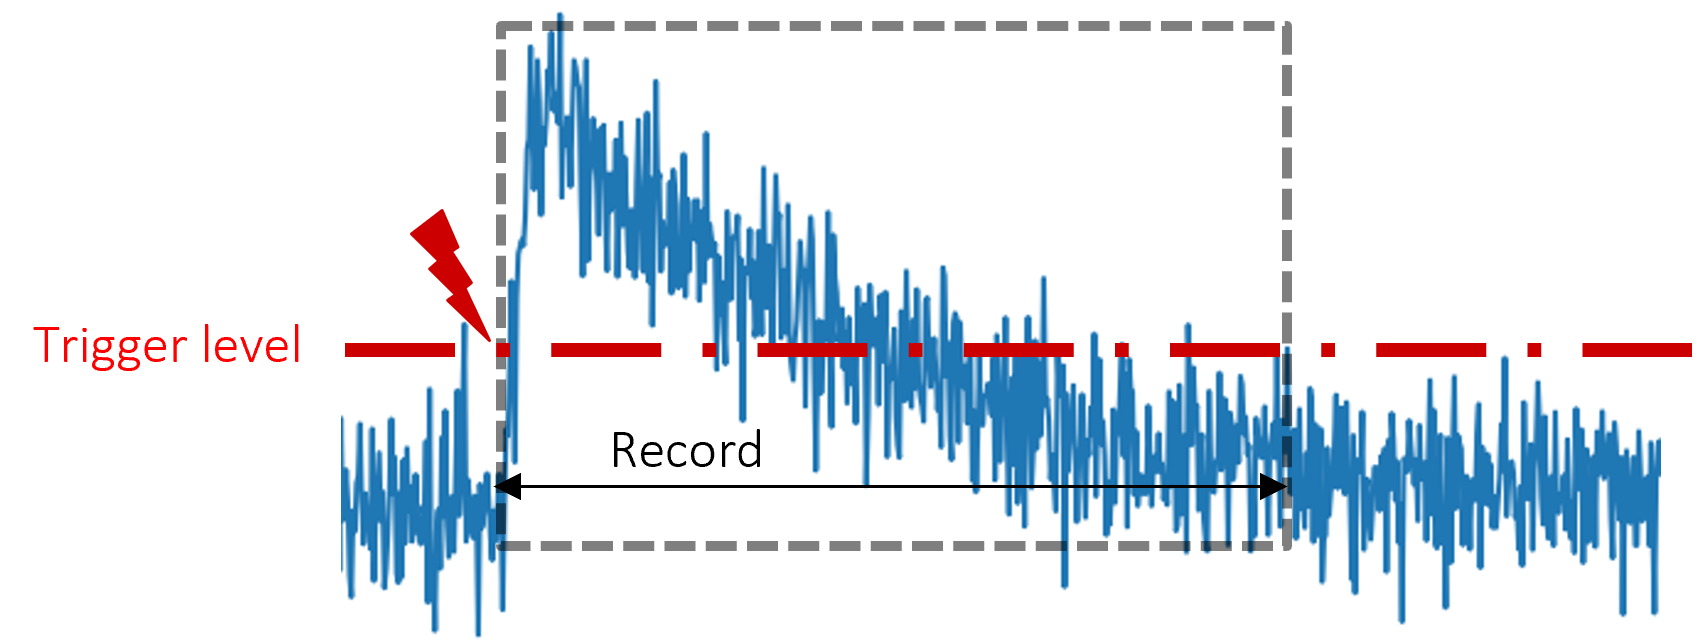
\includegraphics[width=.7\linewidth]{media/level_trigger.png}
  \caption{Level trigger}
  \label{fig:level_trigger}
\end{figure}


Once a window finishes, no more events are detected
until the signal returns to a value below the trigger level
(for rising edge triggering). This reset value might be 
set to be equal to the trigger level, however such approach
might lead to a scenario shown in \autoref{fig:lt_no_hysteresis}.
In a noisy environment the signal might falsely trigger immediately after
a window ends due to a random high spike on the slower falling edge of
an exponential pulse.
\begin{figure}[H]
  \centering
  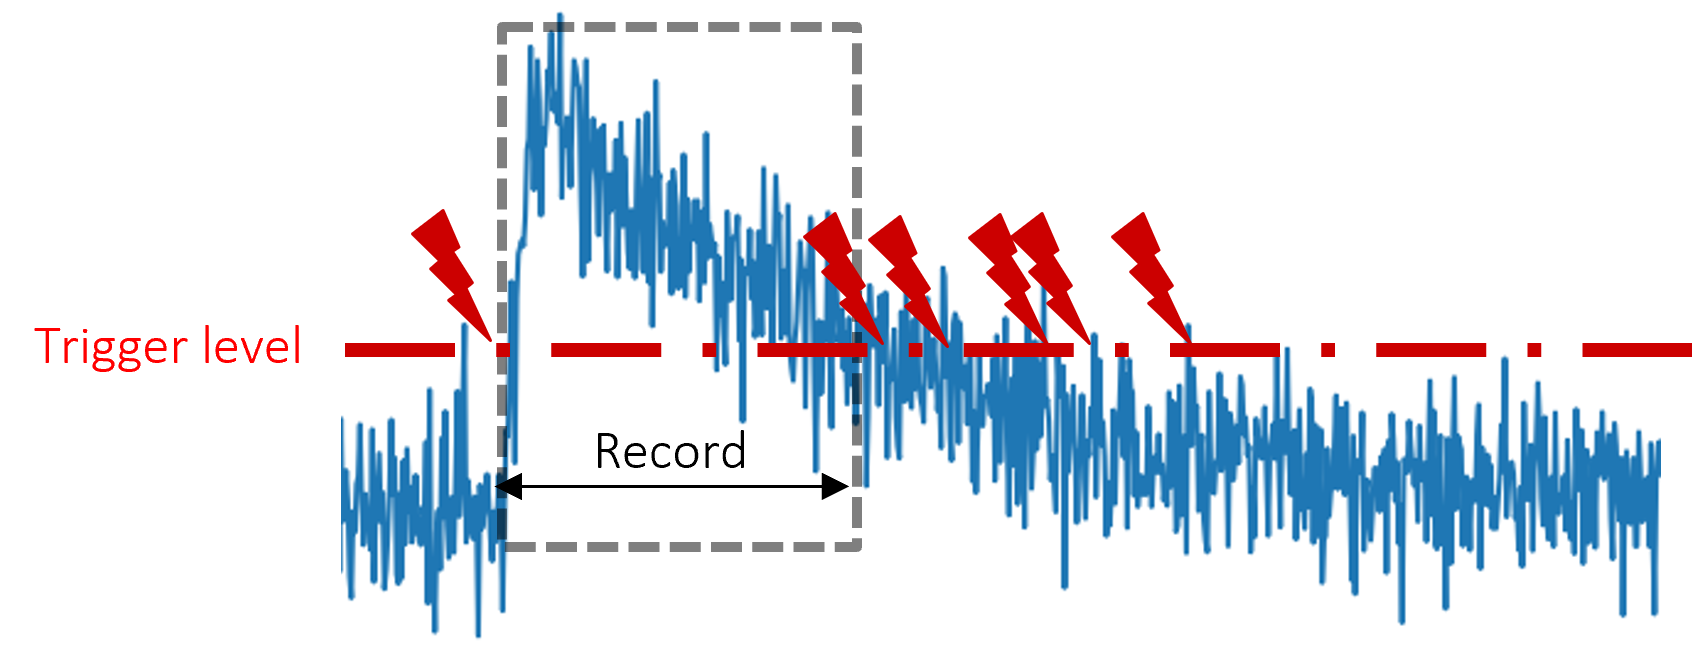
\includegraphics[width=.7\linewidth]{media/lt_no_hysteresis.png}
  \caption{Level trigger with no hysteresis}
  \label{fig:lt_no_hysteresis}
\end{figure}


To prevent such false triggers typically some form of a hysteresis is used.
The reset level is shifted downwards, so that the input signal must cross
a second threshold before the another trigger can be raised.
This threshold should be set to such value, that random noise is guaranteed
to never cause false triggers, but not any lower.
\autoref{fig:lt_hysteresis} shows a hysteresis mitigating some false triggers.
Some of the false triggers from \autoref{fig:lt_no_hysteresis} are removed, however 
due to the high noise some still persist.
\begin{figure}[H]
  \centering
  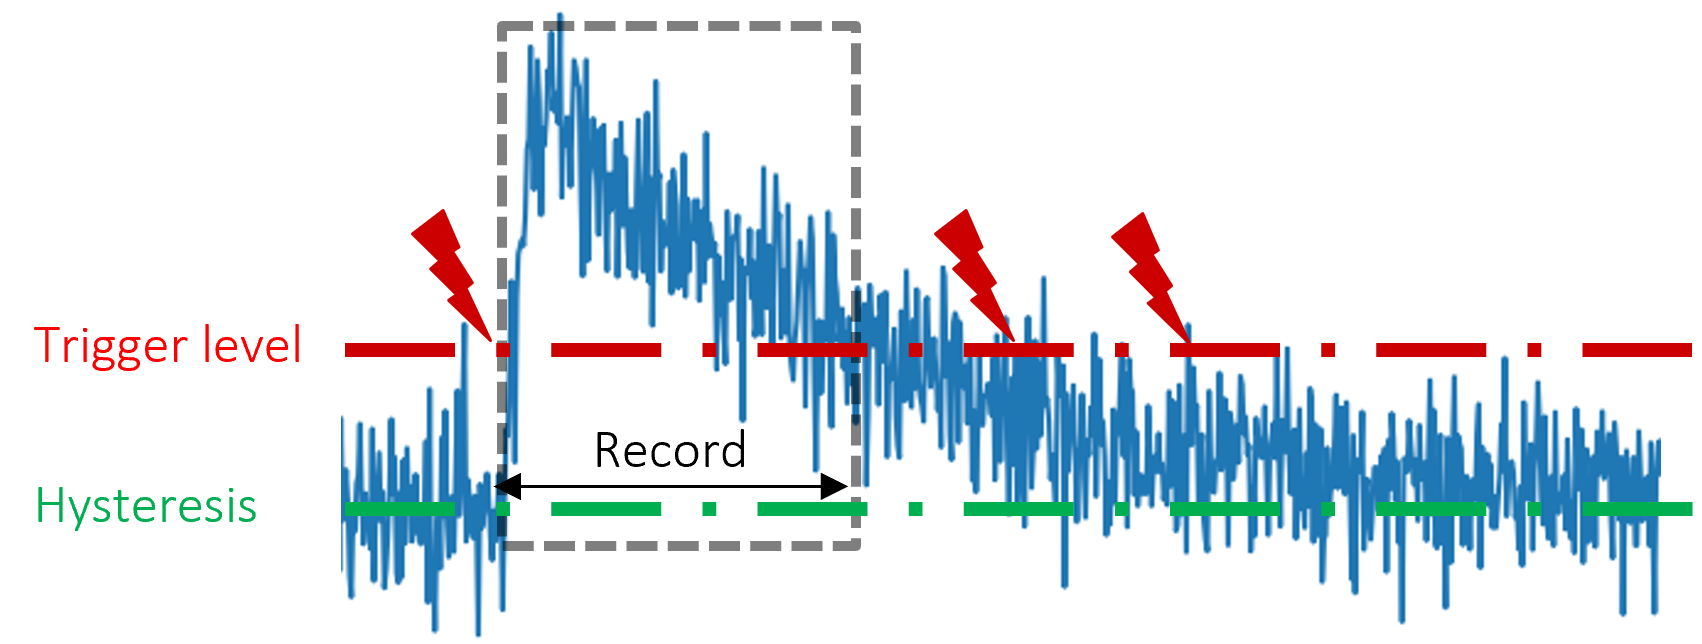
\includegraphics[width=.7\linewidth]{media/lt_hysteresis.png}
  \caption{Level trigger with a hysteresis}
  \label{fig:lt_hysteresis} 
\end{figure}


With the slow falling edge of a pulse, care must be taken not to 
overestimate the hysteresis. By setting the reset level too far away
from the trigger level pile-ups can be missed as pointed in
\autoref{fig:lt_hysteresis_miss}. With a properly set hysteresis
the level trigger offers performance that is sufficient in most applications.
In a tokamak's environment, however, the hysteresis
alone could potentially prove insufficient due to 
EMI and temperature fluctuations.
\begin{figure}[H]
  \centering
  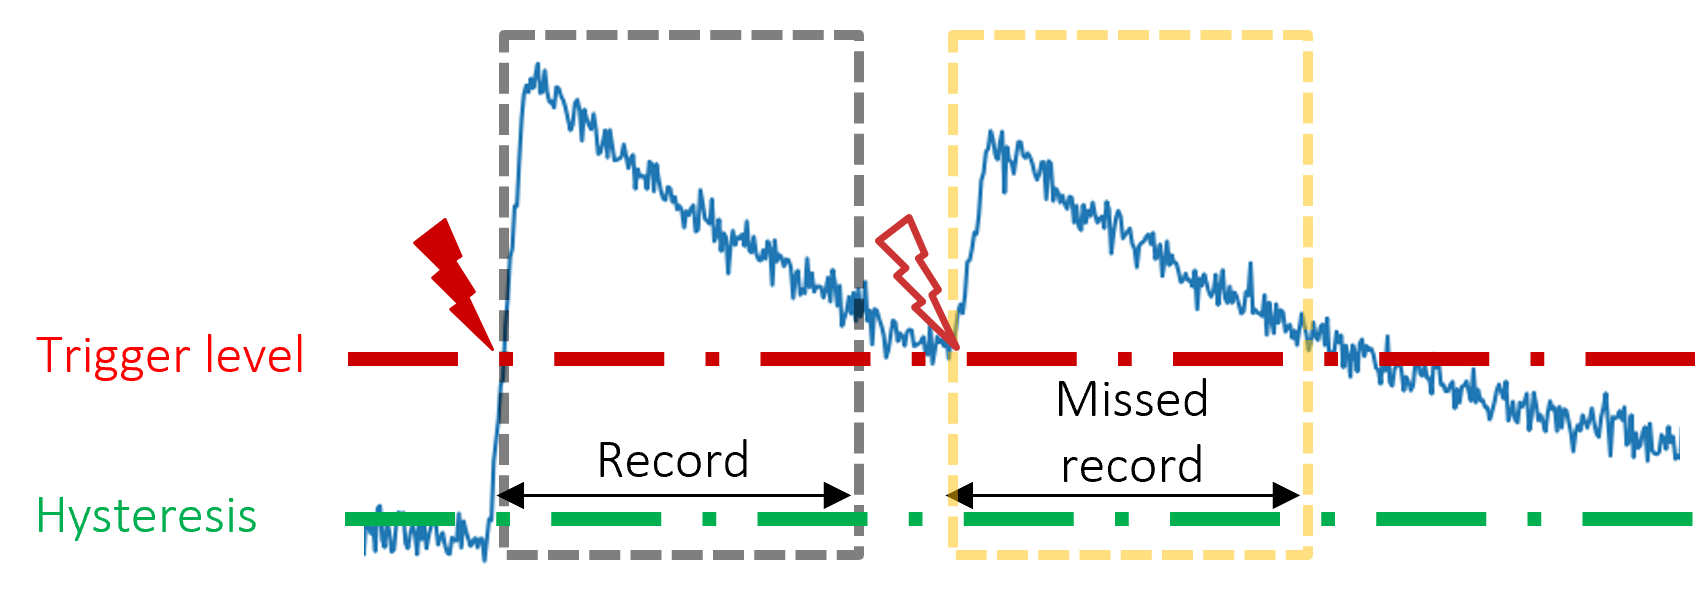
\includegraphics[width=.7\linewidth]{media/lt_hysteresis_miss.png}
  \caption{Level trigger hysteresis causing missed events}
  \label{fig:lt_hysteresis_miss} 
\end{figure}
\subsection{Boxcar filter} \label{ssec:boxcar_filter}


The two problems inherent to simple level triggering 
are its susceptibility to noise and pulse overlap.
Just as with analogue approaches these two problems 
can be minimized with low-pass and high-pass filtering.
By utilizing a low-pass filter the input signal becomes 
smoother, reducing the possibility of 
false triggers caused by random noise spikes. 
A high-pass filter converts the falling edge of a pulse to a sharper curve,
making pile-ups easier to detect.


In the digital domain the simplest filters that perform
these operations are the Moving Average (MA) filter and 
the derivative filter. MA works to reduce the spikes and increase 
SNR. The derivative filter can strip the DC component from
a signal, meaning that the sharp rising edges will become
even easier to detect in comparison to the decaying tails.


By combining the concepts of the MA and derivative filters
into a single module a boxcar filter is obtained. 
\autoref{fig:boxcar_effect} shows an example boxcar transfer function,
together with its effect on an input signal of two exponential pulses.
The boxcar filter can be considered
to be a subtraction of two samples averaged with a window
of length $W$ delayed from each other by $W$. 
On \autoref{fig:boxcar_effect} $W=25$.
\begin{figure}[H]
  \centering
  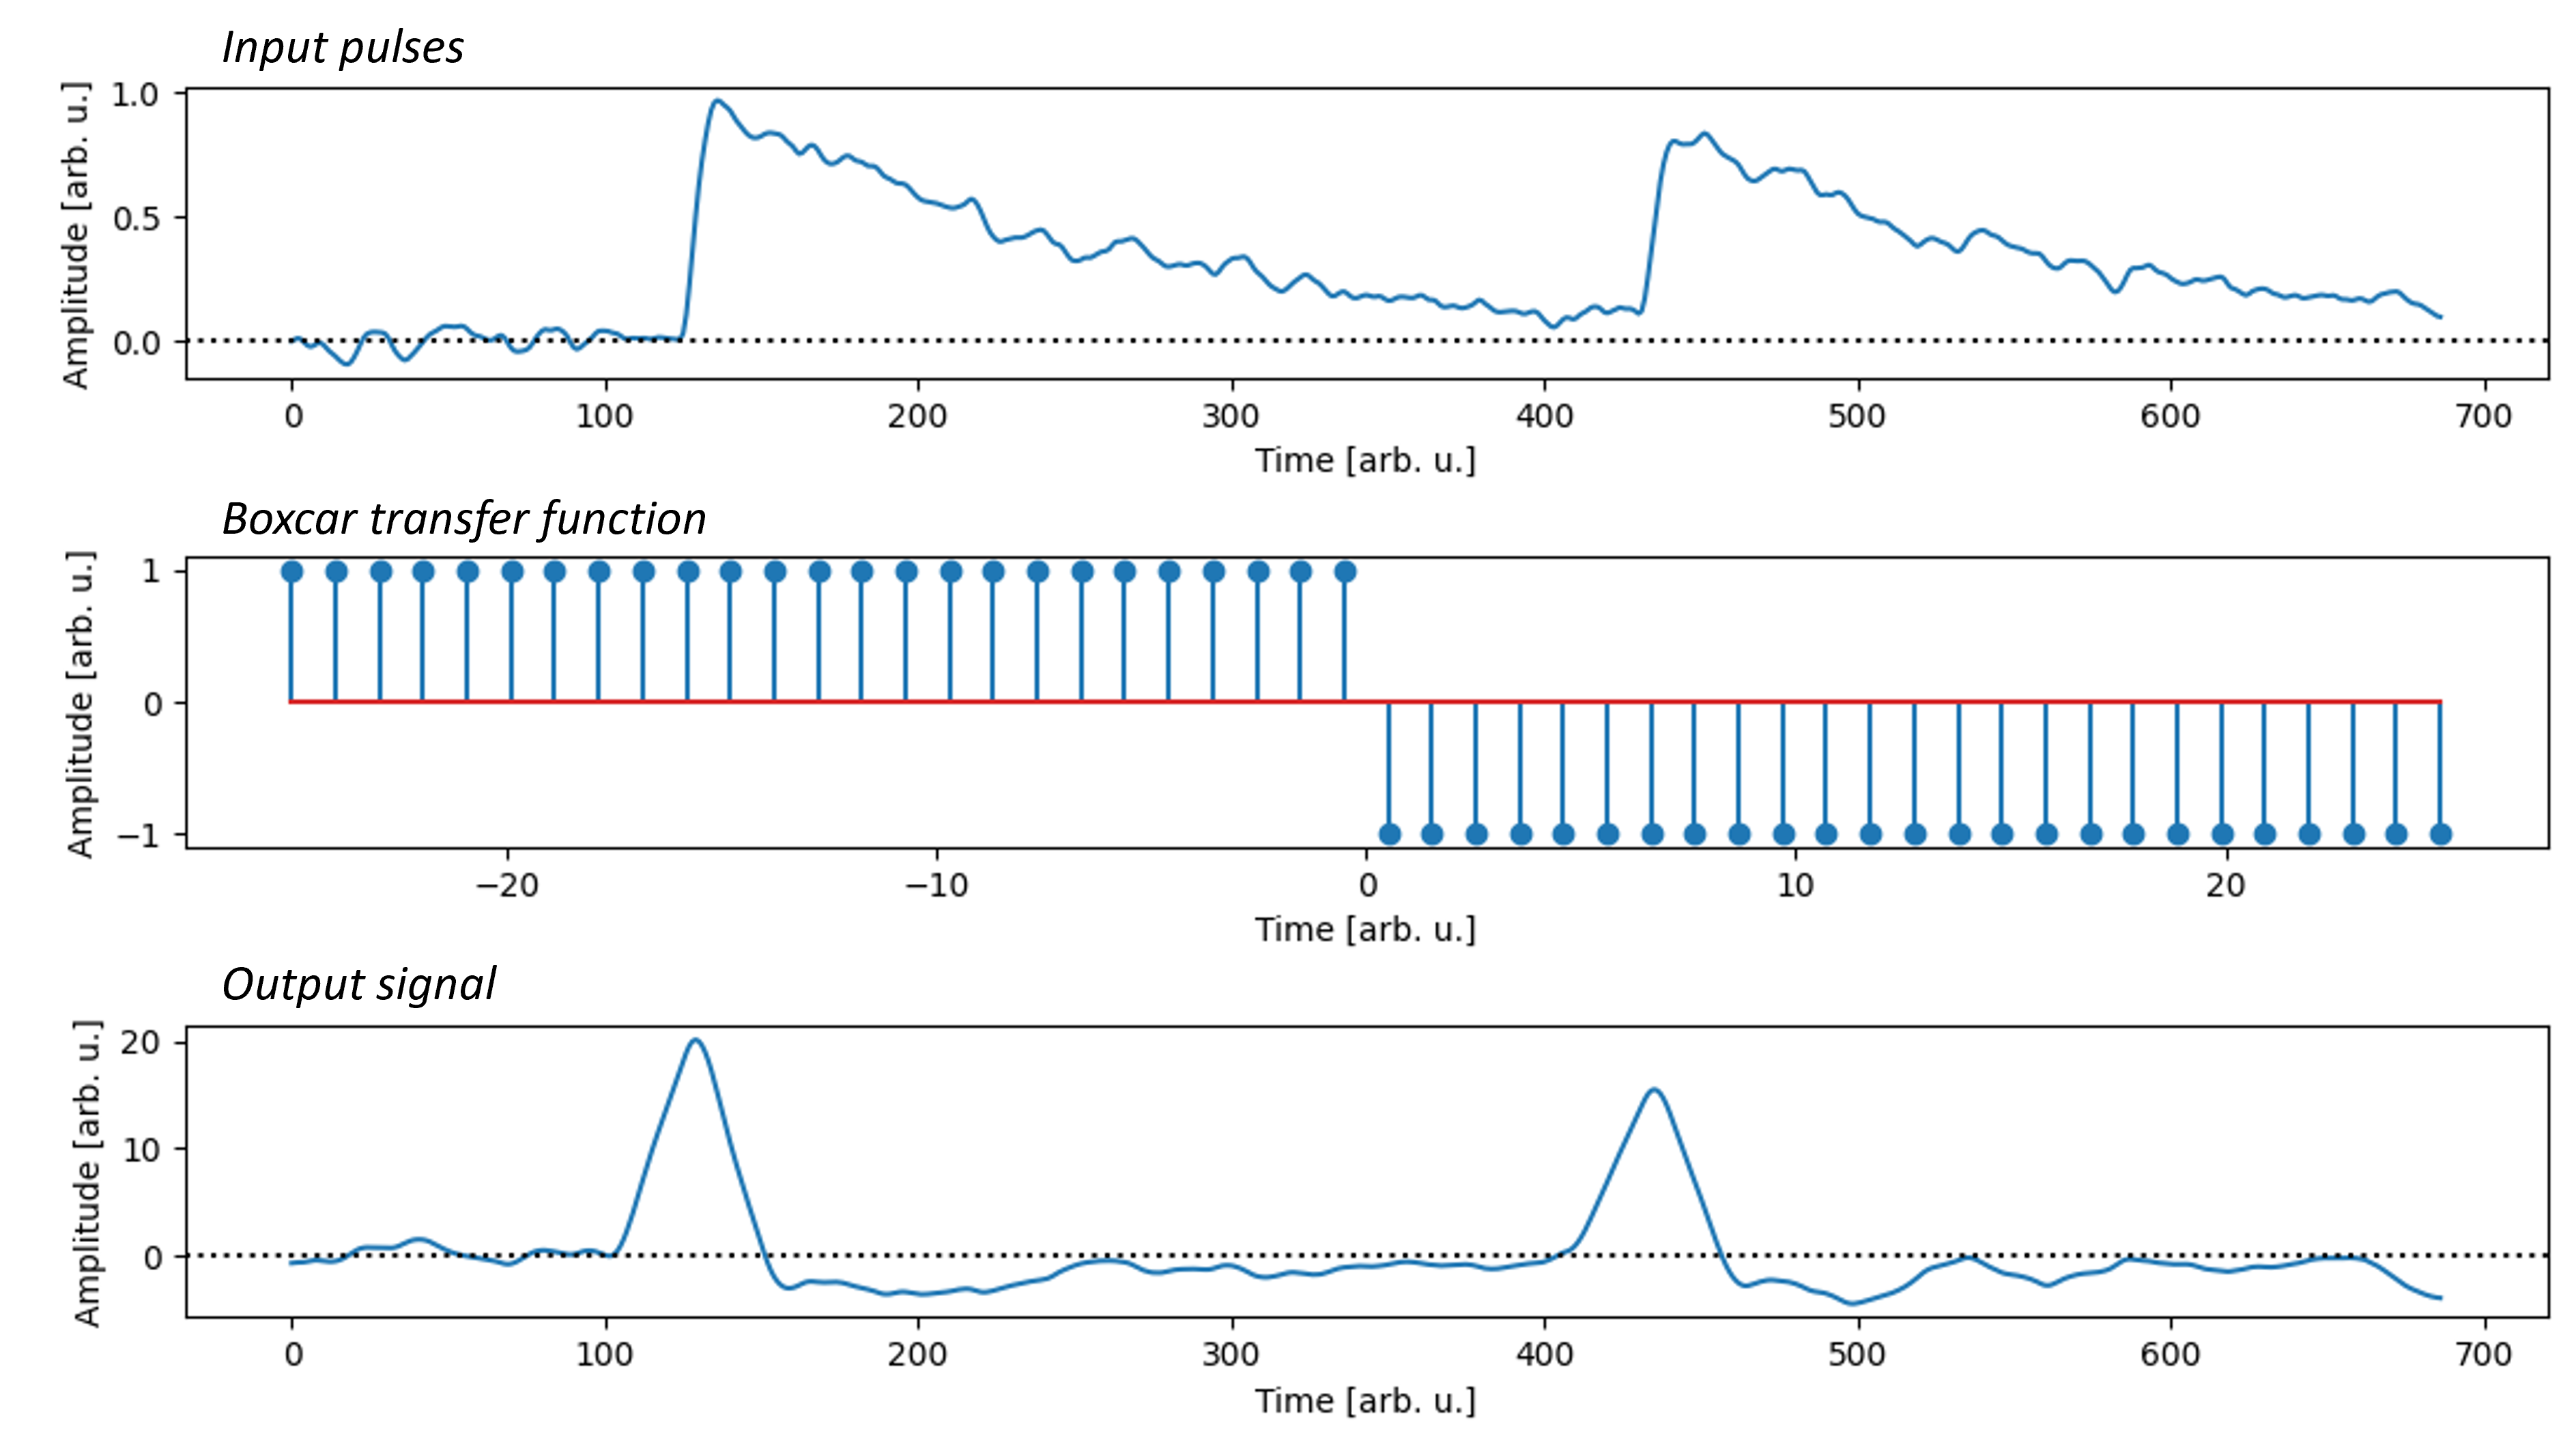
\includegraphics[width=\linewidth]{media/boxcar_effect.png}
  \caption{Effect of boxcar filtering on two exponential pulses}
  \label{fig:boxcar_effect} 
\end{figure}


With level triggering
on the raw pulses the trigger position is the later in a pulse the 
shorter it is. Pulses that reach just slightly above the trigger level
are detected near their top, while pulses significantly stronger
than the trigger level are detected near their start, as shown in 
\autoref{fig:amplitude_walk}. This behaviour is called amplitude walk.

\begin{figure}[H]
  \centering
  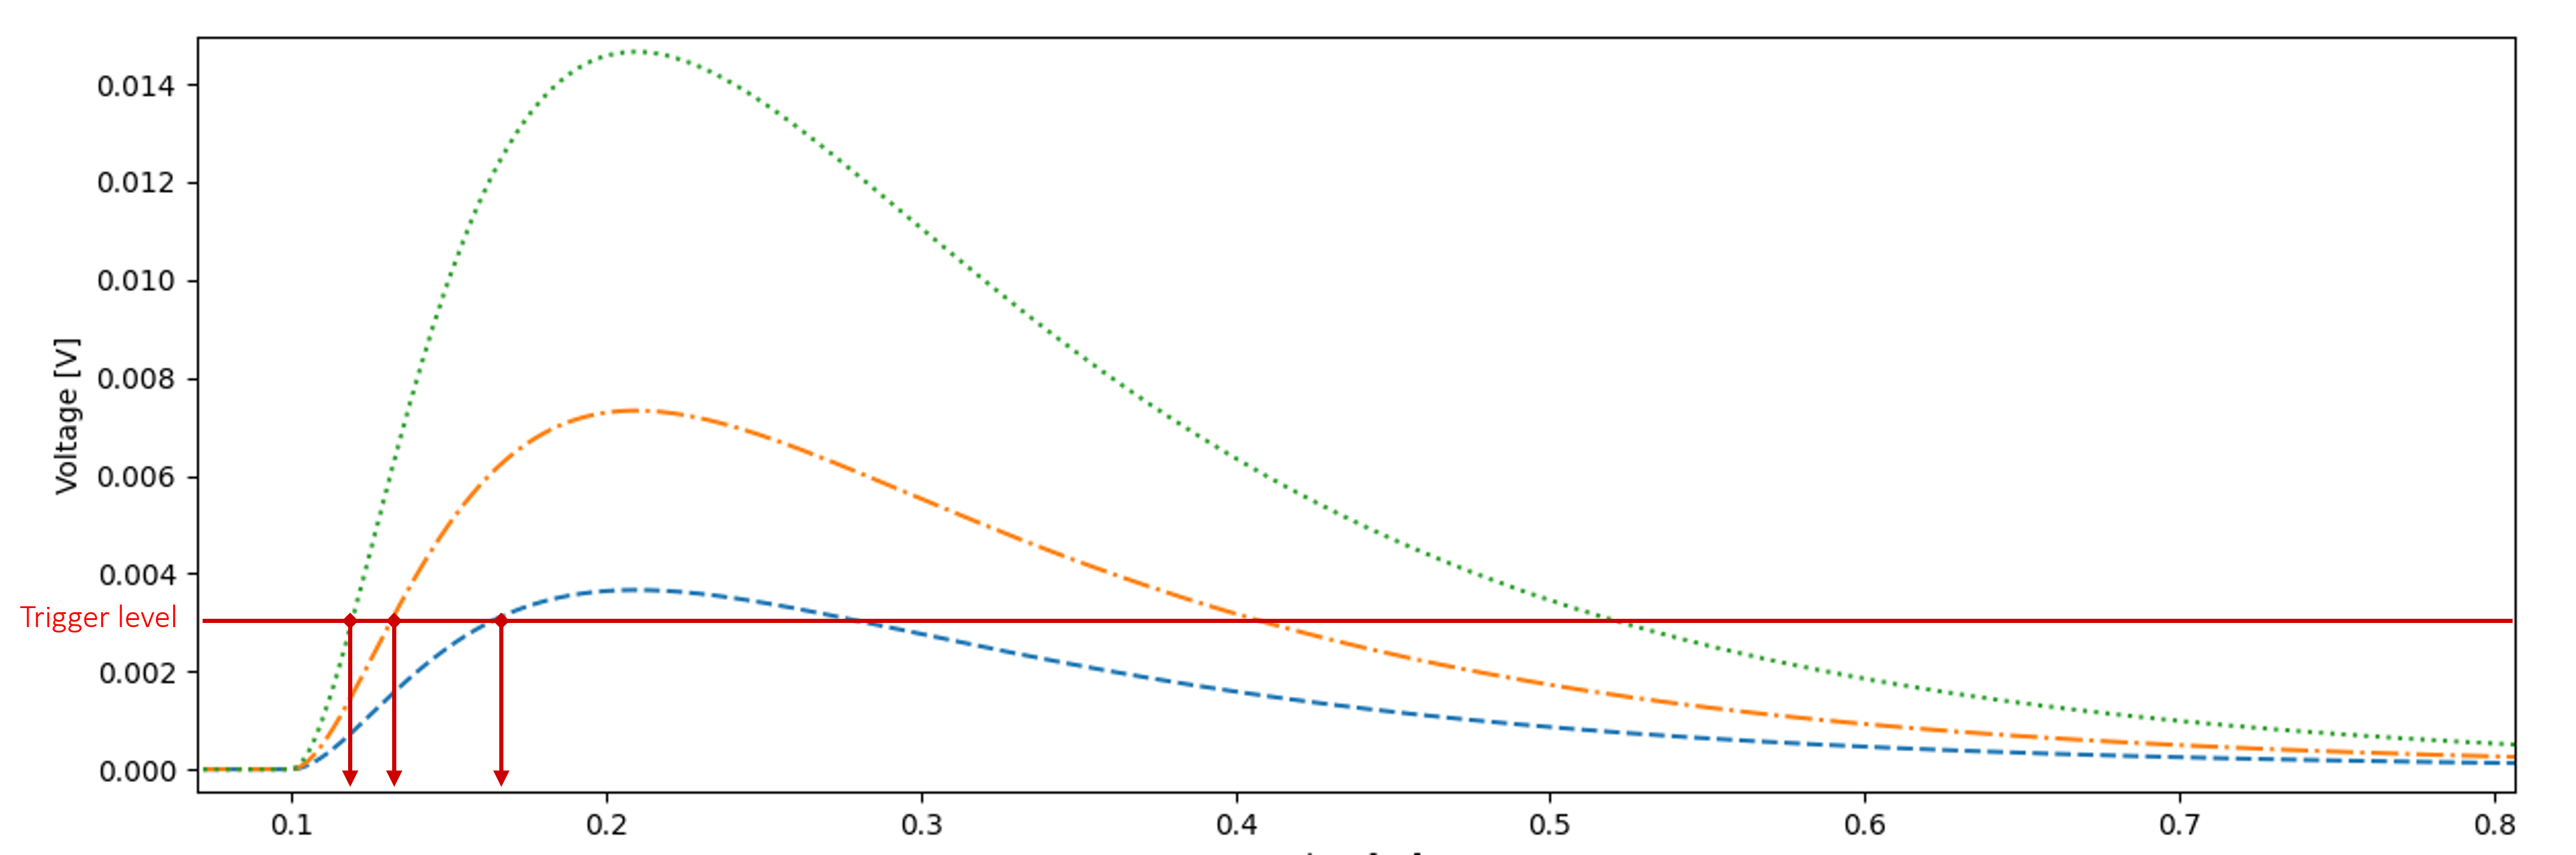
\includegraphics[width=\linewidth]{media/amplitude_walk.png}
  \caption{Amplitude walk}
  \label{fig:amplitude_walk} 
\end{figure}


Due to the differential action of the boxcar filter it can be used in a
digital Constant Fraction Discriminator (CFD).
The point at which a pulse's derivative crosses zero after 
the sharp rise marks the peak of the original pulse. 
When using averaging from the boxcar filter this position 
will be slightly shifted but can still be reliably used to increase
the timestamping precision.

\subsection{Trapezoidal filter}

The trapezoidal filter shapes incoming pulses into the 
shape of an isosceles trapezoid. The sharp rising edge and 
slow decay tail are replaced with same length edges.
Instead of a sharp peak a flattop region is formed that is proportional
to the pulse height. The length of edges and the flattop can be freely
controlled through constants in the filter. \autoref{fig:trapezoid_effect}
shows the effect of a trapezoidal filter being applied to a train
of two exponential pulses. Note the dotted trigger line almost 
causing a false negative if applied to raw signal. 
The filtered signal provides a clear distinction 
between the slightly overlapping pulses.

\begin{figure}[H]
  \centering
  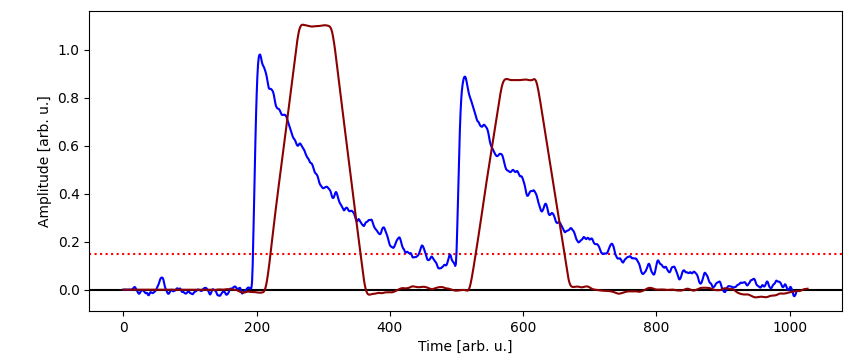
\includegraphics[width=\linewidth]{media/trapezoid_effect.png}
  \caption{Trapezoid filter applied to a train of two pulses}
  \label{fig:trapezoid_effect} 
\end{figure}


The trapezoidal filter is a more complicated filter than the boxcar filter.
It relies on the use of Moving Window Deconvolution (MWD),
as first proposed by Georgiev et al. \cite{mwd}.
It is trivial to obtain a trapezoidal shape from a step input function.
The MWD algorithm works to transform an exponentially decaying pulse into 
a step signal. A step function, while perfect for transformations,
is undesirable in continuous mode of operation.
With multiple pulses, the output of a MWD forms a staircase that quickly saturates.
The simple solution is to perform a subtraction of a delayed sample.
This changes the step signal
to a rectangular shape with a length defined by the delay amount.
The staircase then becomes a train of rectangular pulses.
\autoref{fig:mwd_staircase} shows the consecutive steps of a MWD algorithm.

\begin{figure}[H]
  \centering
  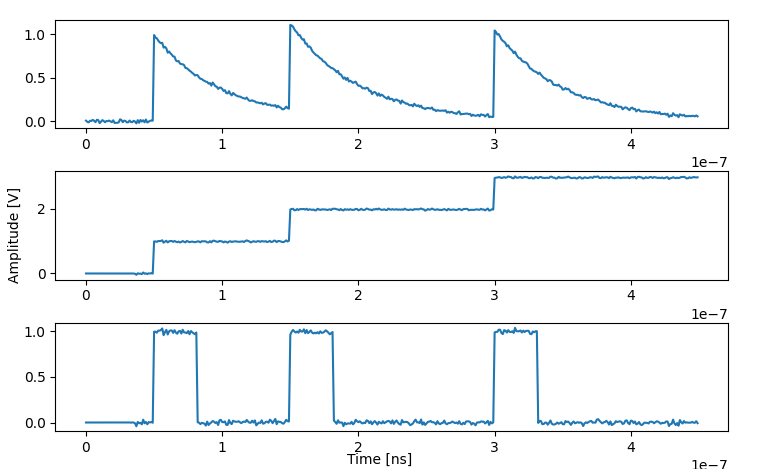
\includegraphics[width=\linewidth]{media/mwd_staircase.png}
  \caption{MWD algorithm applied to a series of 3 pulses}
  \label{fig:mwd_staircase} 
\end{figure}


MWD requires the precise value of the pulse decay constant to
be known. \autoref{fig:mwd_tau} shows the effect of using a wrong value
when configuring the MWD filter. By tuning the filter with a time constant
that is too high an undershoot is obtained after the rectangular shape.
Using a value that is too low causes an overshoot.
Both mistakes reduce the accuracy of pile-up discrimination, 
as consecutive pulses will overlap with the decaying region
and cause imprecise height measurement.

\begin{figure}[H]
  \centering
  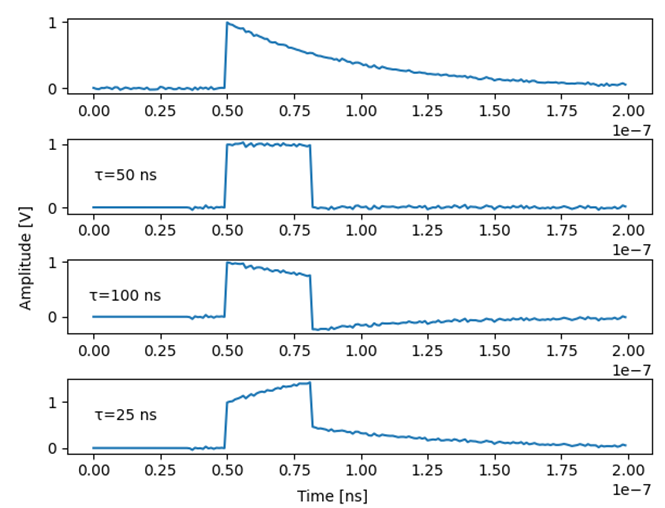
\includegraphics[width=\linewidth]{media/mwd_tau.png}
  \caption{The effects of decay constant mismatch between a pulse and a MWD algorithm. Decay constant of pulses is 50 ns.}
  \label{fig:mwd_tau} 
\end{figure}

The MWD algorithm itself produces a rectangular shape. To obtain a trapezoid
an averaging step is applied. This causes the edges to smoothen and as a 
side effect decrease the noise as shown in \autoref{fig:mwd_average}.
The trapezoid filter can also be synthesized using
alternative methods that are better optimized for hardware implementation
\cite{jordanov_trapezoidal}.
MWD itself requires division which is an extremely resource consuming operation 
in digital signal processing.

\begin{figure}[H]
  \centering
  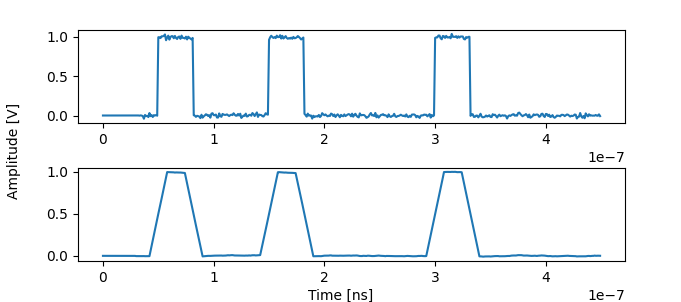
\includegraphics[width=\linewidth]{media/mwd_average.png}
  \caption{Last step of synthesizing a trapezoid with the use of MWD}
  \label{fig:mwd_average} 
\end{figure}

\subsection{Triangular filter}

As mentioned earlier the flattop region of a trapezoidal filter
is not particularly useful for pulse detection. By using an 
averaging filter with the same window length as the MWD window, 
the flattop is squeezed together and a triangular shape is formed
as shown in \autoref{fig:triangular_filter}.
Thus, the triangular filter is a special case of the 
trapezoidal filter that can be used if only detection or timing is of interest.

\begin{figure}[H]
  \centering
  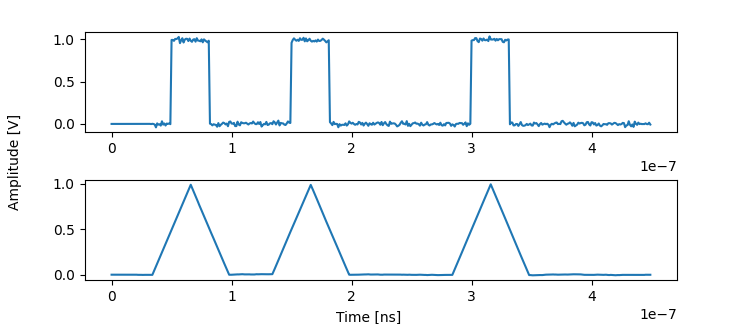
\includegraphics[width=\linewidth]{media/triangular_filter.png}
  \caption{Triangular filter being formed as the last step of a MWD}
  \label{fig:triangular_filter} 
\end{figure}

\subsection{Other pulse detection methods}

Other methods and filters for detection apart from those described above
can be found in scientific literature. They have not been chosen
for implementation in this work due to their low maturity,
excessive complexity or subpar performance. 
Low hardware resource usage and minimal delay
were some of the primary parameters considered.
More experimental methods can provide better performance,
but are harder to implement in real-time in firmware.


Faisal et al. used normalized cross-correlation to compare
the similarity of incoming pulses to a predefined ideal template pulse.
The algorithm was implemented in an FPGA at a sampling rate of 250 MS/s.
When compared to level triggering, 
their method improved the probability of correct pulse detection by a factor of 4
when a template obtained from averaging capture pulses was used;
and by a factor of 3 when a simplified square model was used.
\cite{detection_cross_correlation}


Kamleitner et al. analysed and compared a multitude
of different edge detection algorithms. 
Apart from algorithms similar to the trapezoidal filter and the boxcar
filter described above, the work analyzed three similarity matching algorithms,
Canny's edge detector, as well as a few optimally designed FIR filters.
The optimum filters won the proposed benchmarks, however, they were closely followed by
the boxcar-like Single Delay Line, as well as the trapezoidal filter.
Similarity filters fared significantly worse, offering superior performance
only when it came to the number of false positives.
\cite{pulse_processing_methods}

\subsection{Simulation performance}

In order to find the most suitable filters for hardware implementation
in the Hard X-Ray Monitor the algorithms were first subjected to a
series of simulated software tests.
Level triggering, zero crossing detection, triangular and boxcar 
filtering were implemented with the use of the numpy and scipy
libraries in Python. 
The same libraries were used to create a test bench for generating
simulated impulses with a configurable frequency, noise, amplitude and decay constant.


The test pulse trains were fed to the filters and each output was 
tested with an array of different trigger configurations.
The trigger level and reset at which there was the least amount of mistakes for
a given algorithm was chosen as the representative record for comparison
between different filters.
For each record the number of properly detected pulses (true positives),
missed pulses (false negatives) and noise mistaken for pulses (false positives) 
were counted and divided by the total pulse count.
This was done, because the pulse count was higher in tests that checked 
the behavior under high pile-up conditions.


For initial functionality tests and debugging, a graphical user interface
was prepared with the use of the matplotlib library.
The tool would run a test scenario, generate a train of pulses with 
the specified parameters, filter the input signal and run
user-configured level triggering on the output signal.
The end result would be a plot superimposing the input and output signals.
Detected pulse were marked with a green rectangle. Missed pulses
showed up as red dashed rectangles and badly classified noise
was marked with an orange color. \autoref{fig:graphical_tool_boxcar}
shows an example output from the graphical tool. A boxcar filter is used 
to improve the performance of detection. In the example one pulse
is not detected due to pile-up and one is not detected due
to a badly configured trigger threshold.

\begin{figure}[H]
  \centering
  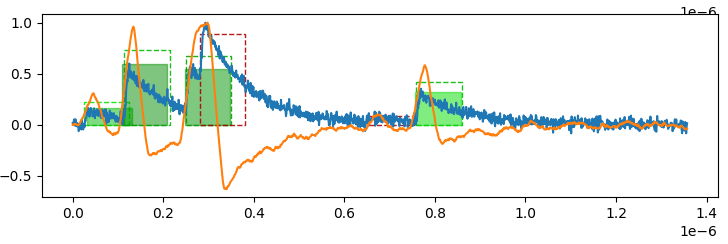
\includegraphics[width=\linewidth]{media/graphical_tool_boxcar.png}
  \caption{Example output from the graphical tool for debugging detection filters}
  \label{fig:graphical_tool_boxcar} 
\end{figure}

Once the filters and the testbench were rid of bugs and optimized 
with the graphical tool, the code was modified for automated testing.
Instead of using user-specified trigger levels the script would 
test a range of settings to find the best ones. In place of the graphical
result a confusion matrix for each detection approach was given.
The best results from each algorithm were then plotted on
one graph to obtain a figure of merit based comparison for 
different methods.


\autoref{fig:detection_sim_pulse_rate} and \autoref{fig:detection_sim_noise}
show the results of the simulations. The cost function used to rate the 
filters was a sum of false negatives and false positives divided by the 
total number of pulses that actually were present in the simulation.
Both triangular and boxcar filters provide an immense improvement over
level triggering on untreated signal. A triangular filter
with the same max delay length provides slightly better accuracy 
than a boxcar filter.


While a filter with a longer averaging effect (longer window length) 
fares better in noisy environments, as indicated in figure
\autoref{fig:detection_sim_noise}, the inverse is true when 
it comes to pile-up frequency. Shorter filters have a higher likelihood
of discriminating between two overlapping pulses as shown 
by the results in \autoref{fig:detection_sim_pulse_rate}.
There is no single detection filter that is best suited for all applications.
The filter must be tuned to a specific use case, however
some filters, like the boxcar offer a simpler interface for
doing so, than others.

  \begin{figure}[H]
    \centering
    \begin{minipage}{.45\textwidth}
      \centering
      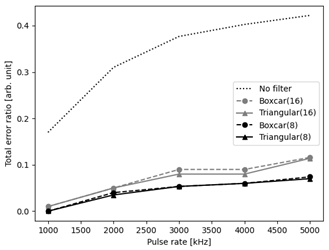
\includegraphics[width=\linewidth]{media/detection_sim_pulse_rate.png}
      \caption{Detection algorithms compared under varying pulse frequency}
      \label{fig:detection_sim_pulse_rate}
    \end{minipage}%
    \hfill
    \begin{minipage}{.45\textwidth}
      \centering
      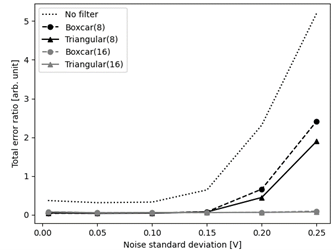
\includegraphics[width=\linewidth]{media/detection_sim_noise.png}
      \caption{Detection algorithms compared under varying noise magnitude}
      \label{fig:detection_sim_noise}
    \end{minipage}
  \end{figure}
